% assignment_2.tex
% CS 8735 - Unsupervised Learning (Fall 2015)
%     University of Missouri-Columbia
%             Chanmann Lim
%            October 2015

\documentclass[a4paper]{article}

\usepackage[margin=1 in]{geometry}
\usepackage{listings}
\usepackage{amsmath}
\usepackage{graphicx}
\usepackage{float}
\usepackage{multirow}

\everymath{\displaystyle}
\DeclareMathOperator*{\argmax}{\arg\!\max}
\DeclareMathOperator*{\argmin}{\arg\!\min}

\begin{document}
\noindent The Matlab code for all experiments is in the \textbf{Appendix} section.

\paragraph{6.} Hello

\begin{figure}[H]
  \centering
    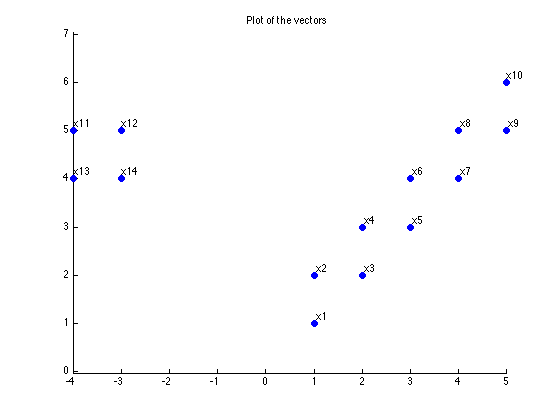
\includegraphics[scale=.57]{images/vectors.png}
  \caption{Plot of vectors}
  \label{fig:vectors}
\end{figure}

\newpage
\subsection*{Appendix:}
	\lstinputlisting[language=Matlab, title=\lstname, basicstyle=\footnotesize]{assignment_2.m}
	\lstinputlisting[language=Matlab, title=\lstname, basicstyle=\footnotesize]{problem_6.m}
	\lstinputlisting[language=Matlab, title=\lstname, basicstyle=\footnotesize]{bsas.m}
	\lstinputlisting[language=Matlab, title=\lstname, basicstyle=\footnotesize]{mbsas.m}
	\lstinputlisting[language=Matlab, title=\lstname, basicstyle=\footnotesize]{min_distance.m}
	\lstinputlisting[language=Matlab, title=\lstname, basicstyle=\footnotesize]{print_cluster.m}
\end{document}